To assess the effectiveness of our extended framework, we begin by replicating the intrinsic homotopy experiment from Chan et al.~\cite{chang_clust_met_space}.
Our goal is to directly compare the representational alignment achieved by affine and non-linear transformations.

We aimed to reproduce the results reported in the original work as closely as possible.
In a first attempt, we applied the architecture and loss computation as described in the original paper, and used the train data for training and test data for evaluation. 
However, this setting did not yield meaningful approximation of the target representations.
In a second attempt, we trained the transformations on the training set, again using the original architecture and per-sample maximum loss. This setup led to a close reproduction of the results reported in the paper: for most tasks, we observed very similar approximation distances on the training set. The only deviations were slightly lower distances for \texttt{SST-2} and slightly higher values for \texttt{RTE}, as measured by the median.
Figure~\ref{fig:baseline-reproduction-trainings-loss} confirms that our reimplementation closely matches the reported training performance

\begin{figure}[h]
	\centering
	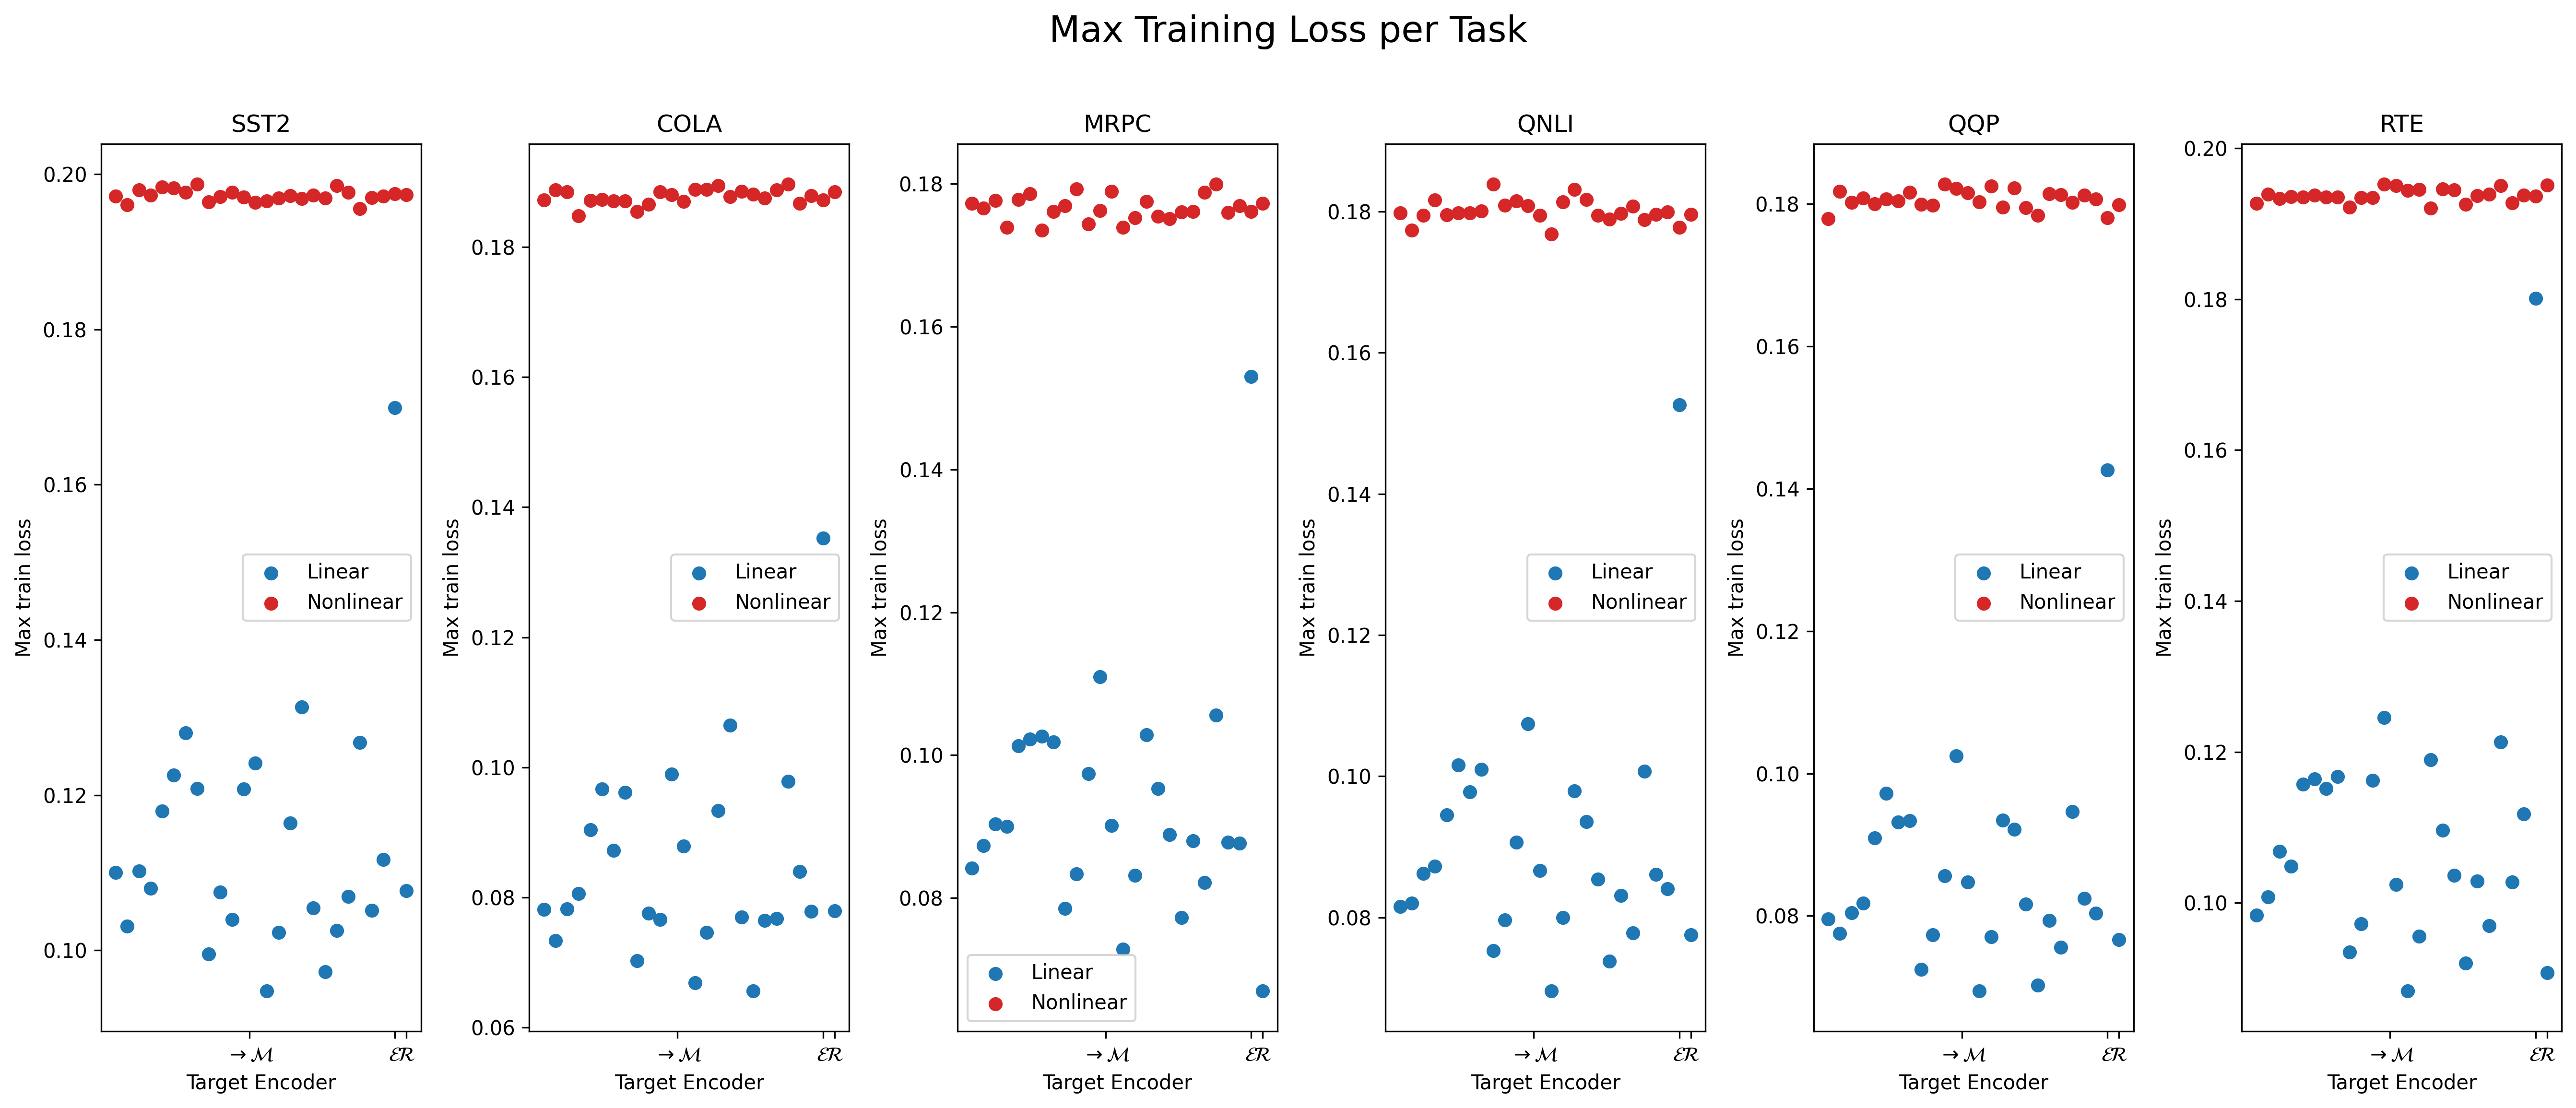
\includegraphics[width=\linewidth]{Abschlussarbeit/Pictures/New_all_in_one_scatter_lower_height.png}
	\caption{Intrinsic approximation distances on the training set for affine and non-linear transformations under the original training scheme.}
	\label{fig:baseline-reproduction-trainings-loss}
\end{figure}

To ensure a rigorous and transparent evaluation protocol for the subsequent experiments, we now consistently train on the training split, use early stopping based on validation loss, and report final results on a held-out test set.

After verifying that our implementation reproduces the reported approximation behavior on the training set, we next examine the intrinsic homotopy distances across a range of learning rates for both affine and non-linear transformations.

In Section~\ref{IH}, we formalized the concept of intrinsic homotopy using linear mappings \( \psi \in S \subset \text{Aff}(V) \), and in Section~\ref{InrinsicHomotopyonNonlinTransf} extended this framework to the nonlinear case \( \psi \in  \mathcal{F}_{\text{Lip}_1} \subset \mathcal{C}_{V,W} \), where \(  \mathcal{F}_{\text{Lip}_1} \subset \mathcal{C} \) consists of 1-Lipschitz continuous neural networks.

To empirically compare the representational alignment induced by these transformation classes, we compute the intrinsic homotopy distances \( d_{\mathrm{Aff}} := d_{\mathcal{\text{Aff}}}(h, g) \) and \( d_{\mathcal{F}_{\mathrm{Lip}_1}} := d_{\mathcal{F}_{\mathrm{Lip}_1}}(h, g) \) for each pair of encoders \( h, g \in \mathcal{E}_V \).
The mean of all distances is visualized for each learningrate and task in Figure~\ref{fig:lin_vs_nonlind_dist}.

\begin{figure}[h]
    \centering
    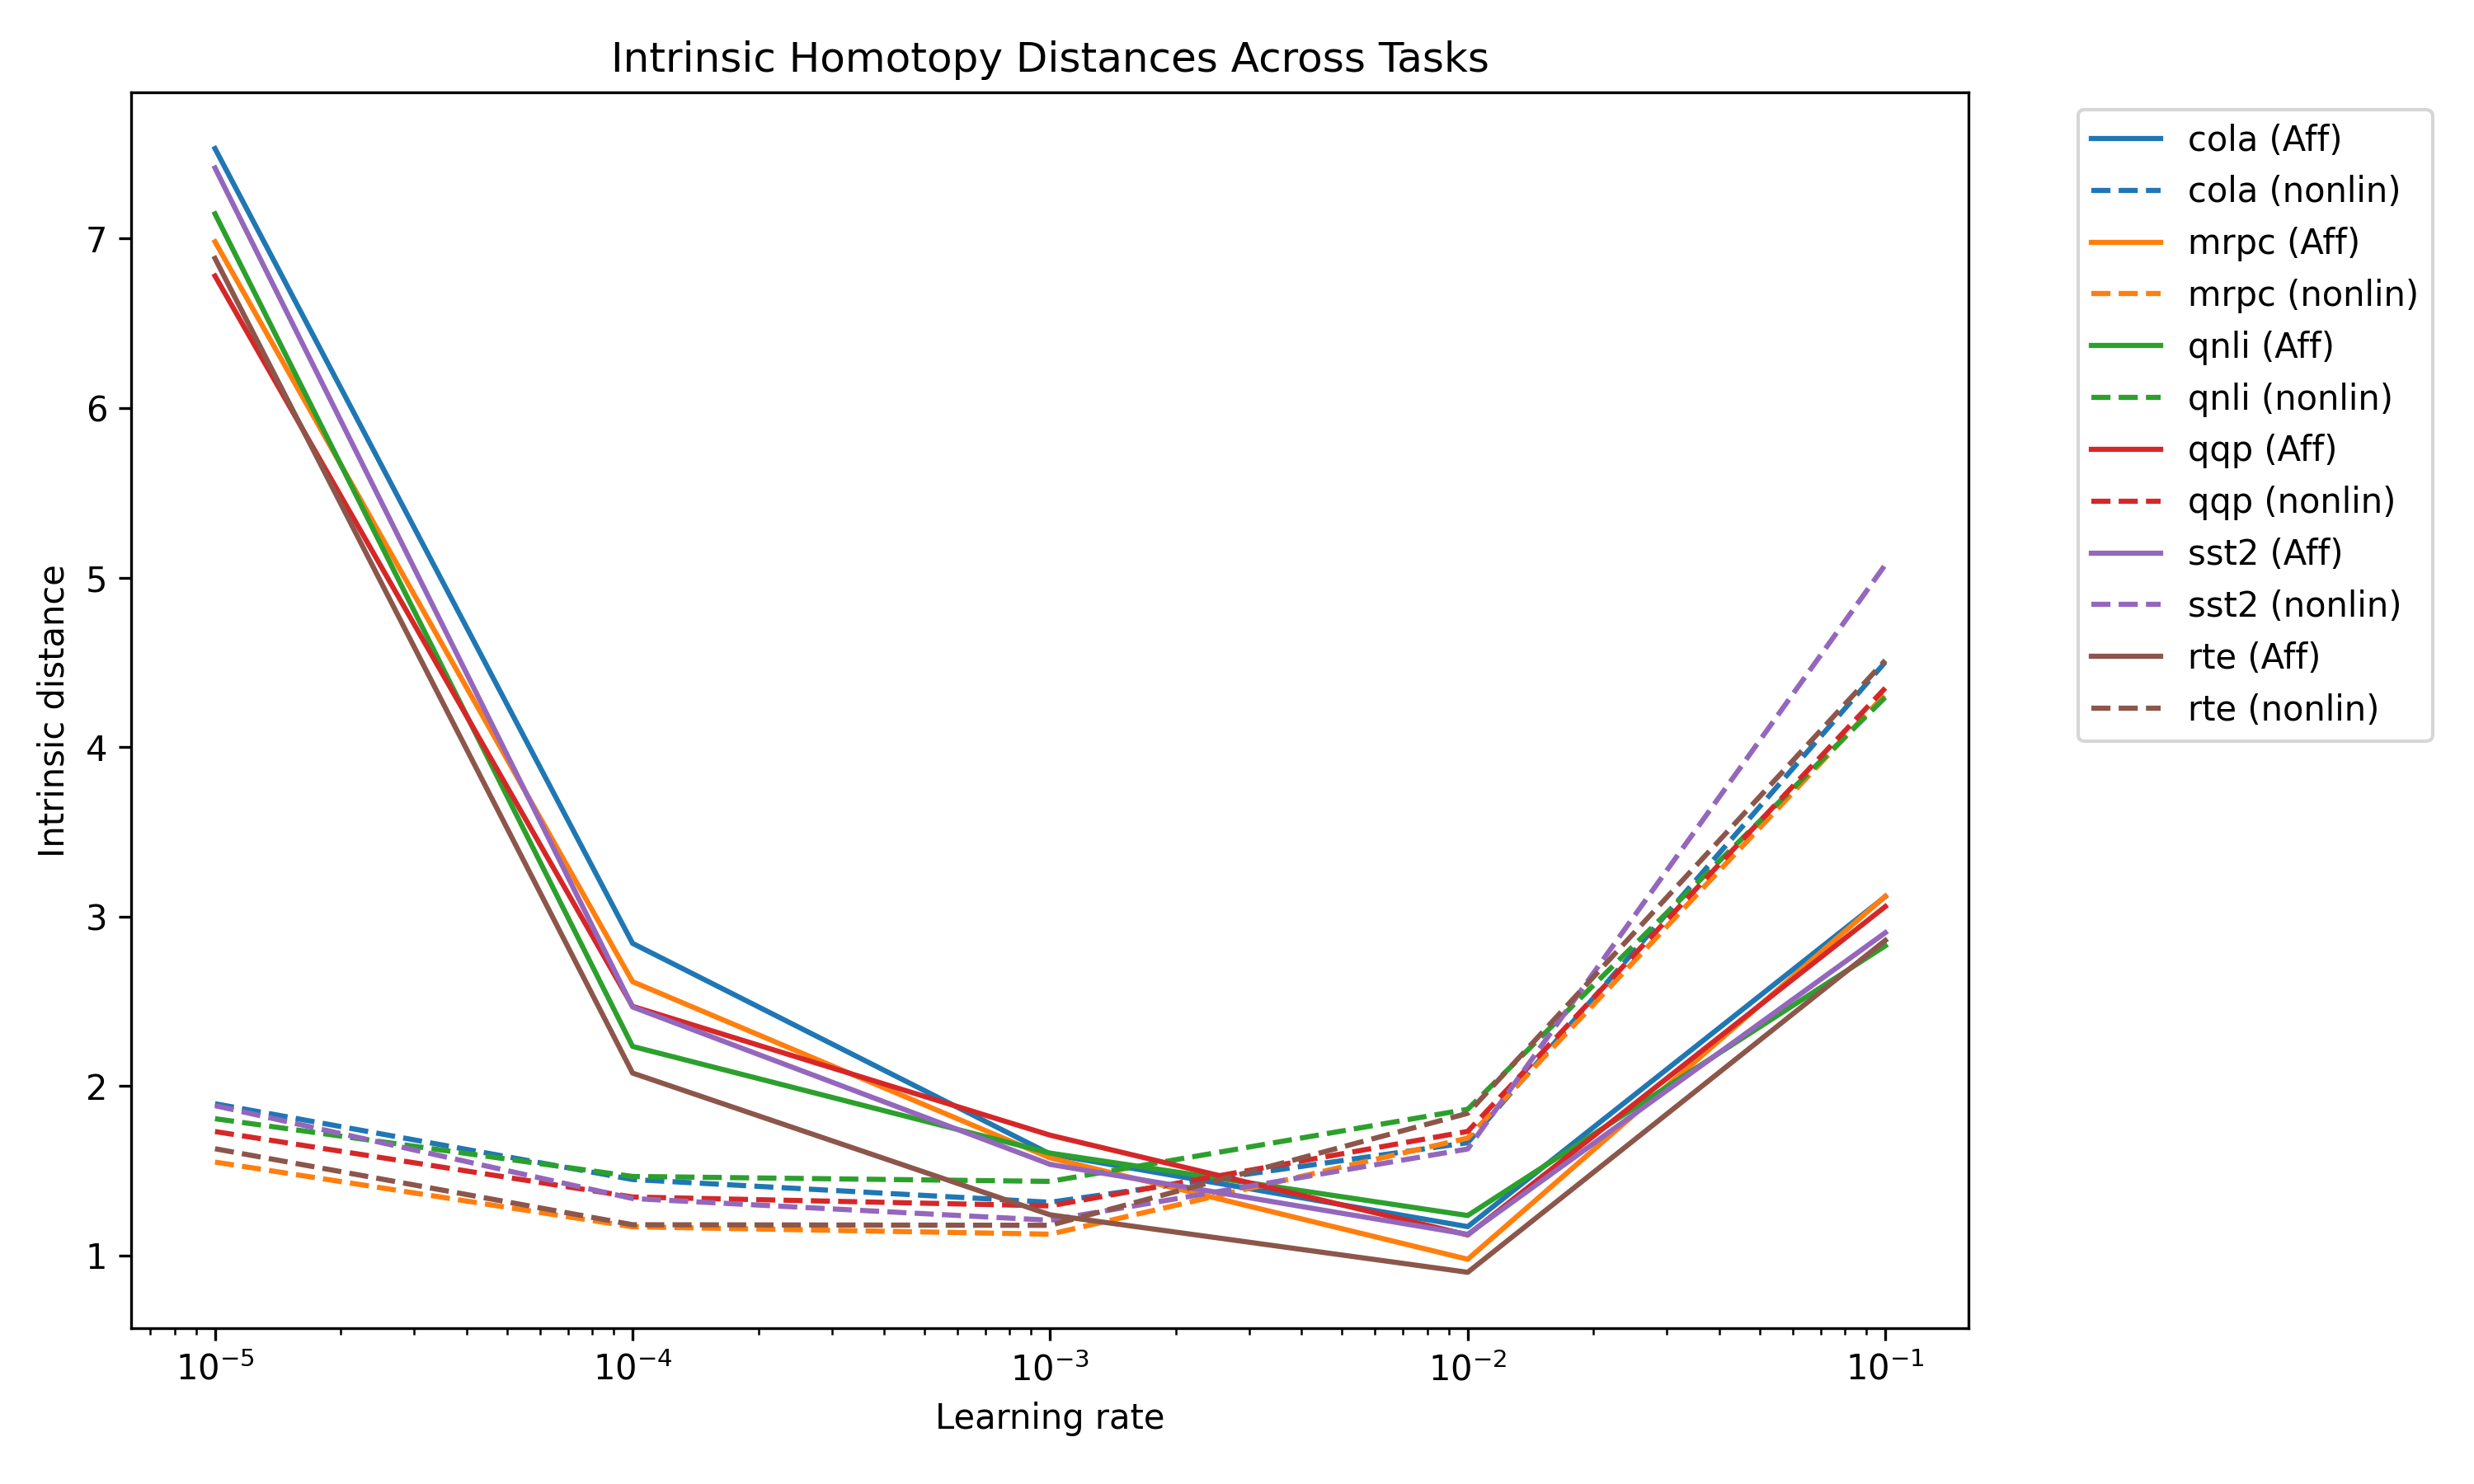
\includegraphics[width=\linewidth]{Abschlussarbeit/Pictures/intrinsic_distance_all_tasks.png}
    \caption{Intrinsic Distances across tasks and learning rates for linear and non-linear models}
    \label{fig:lin_vs_nonlind_dist}
\end{figure}

In addition to the homotopy distances, we report Spearman’s $\rho$ and Pearson’s $r$ correlations between predicted and target representations for both transformation regimes in Table~\ref{tab:correlation-transposed}.  
These metrics serve as complementary indicators of representational alignment: while the homotopy distance measures global approximation quality, the correlation coefficients quantify local relational consistency between vector pairs.

Spearman’s $\rho$ captures the rank-order correlation between the transformed representation $\psi(g)$ and the target $h$. 
As a rank-based measure, it is robust to monotonic non-linear distortions and reflects whether the relative structure between examples is preserved.

In contrast, Pearson’s $r$ quantifies the linear correlation between vectors.  
To assess whether a meaningful linear mapping between model representations exists, we compute $r(g, h)$, the Pearson correlation between the hidden states of the source and target models.  
Consistently low values of $r(g, h)$ across all tasks indicate that no strong global linear relationship exists between $g$ and $h$, implying that affine transformations are fundamentally limited in their ability to approximate one encoder from another.


While we include Pearson’s $r$ for interpretability, we do not use it as a basis for comparing model performance across tasks.

\begin{table}[h]
\centering
\caption{Correlation scores \(\rho, r\) across tasks and learning rates for linear and non-linear models.}
\label{tab:correlation-transposed}
\begin{tabular}{l c ccccccc}
\toprule
&\textbf{lr} & \texttt{QNLI} & \texttt{CoLA} & \texttt{MRPC} & \texttt{QQP} & \texttt{RTE} & \texttt{SST-2} \\
\midrule
\multirow{5}{*}{\(\rho_{\mathrm{Aff}}\)} 
& \(1\cdot10^{-5}\) & 0.44 & 0.29 & 0.47 & 0.44 & 0.44 & 0.32 \\
& \(1\cdot10^{-4}\) & 0.48 & 0.33 & 0.51 & 0.48 & 0.47 & 0.35 \\
& \(1\cdot10^{-3}\) & 0.47 & 0.33 & 0.51 & 0.47 & 0.47 & 0.35 \\
& \(1\cdot10^{-2}\) & 0.33 & 0.23 & 0.36 & 0.34 & 0.32 & 0.23 \\
& \(1\cdot10^{-1}\) & 0.089 & 0.058 & 0.089 & 0.094 & 0.080 & 0.054 \\
\midrule
\multirow{5}{*}{\(\rho_{\mathcal{C}}\)} 
& \(1\cdot10^{-5}\) & 0.089 & 0.11 & 0.12 & 0.11 & 0.11 & 0.10 \\
& \(1\cdot10^{-4}\) & 0.079 & 0.13 & 0.18 & 0.10 & 0.12 & 0.11 \\
& \(1\cdot10^{-3}\) & 0.026 & 0.079 & 0.0054 & 0.066 & 0.021 & 0.071 \\
& \(1\cdot10^{-2}\) & 0.014 & 0.061 & 0.0037 & 0.043 & 0.012 & 0.049 \\
& \(1\cdot10^{-1}\) & –0.008 & –0.018 & –0.0046 & –0.018 & –0.0051 & –0.023 \\
\midrule
\(r\) 
& &  \(5\cdot10^{-6}\) & \(4\cdot10^{-6}\) & \(4\cdot10^{-6}\) & \(5\cdot10^{-6}\) & \(3\cdot10^{-6}\) & \(5\cdot10^{-6}\)\\
%\multirow{5}{*}{\(r\)} 
%& \(1\cdot10^{-5}\) & \(5.2\cdot10^{-6}\) & \(4.4\cdot10^{-6}\) & \(3.6\cdot10^{-6}\) & \(4.5\cdot10^{-6}\) & \(2.5\cdot10^{-6}\) & \(4.8\cdot10^{-6}\) \\
%& \(1\cdot10^{-4}\) & \(5.2\cdot10^{-6}\) & \(4.4\cdot10^{-6}\) & \(3.6\cdot10^{-6}\) & \(4.5\cdot10^{-6}\) & \(2.5\cdot10^{-6}\) & \(4.8\cdot10^{-6}\) \\
%& \(1\cdot10^{-3}\) & \(5.2\cdot10^{-6}\) & \(4.2\cdot10^{-6}\) & \(3.6\cdot10^{-6}\) & \(4.5\cdot10^{-6}\) & \(2.5\cdot10^{-6}\) & \(4.8\cdot10^{-6}\) \\
%& \(1\cdot10^{-2}\) & \(3.7\cdot10^{-6}\) & \(4.2\cdot10^{-6}\) & \(3.6\cdot10^{-6}\) & \(3.8\cdot10^{-6}\) & \(2.5\cdot10^{-6}\) & \(4.8\cdot10^{-6}\) \\
%& \(1\cdot10^{-1}\) & \(3.7\cdot10^{-6}\) & \(4.2\cdot10^{-6}\) & \(3.6\cdot10^{-6}\) & \(3.8\cdot10^{-6}\) & \(2.5\cdot10^{-6}\) & \(4.8\cdot10^{-6}\) \\
\bottomrule
\end{tabular}
\end{table}

Considering Figure~\ref{fig:lin_vs_nonlind_dist} and Table~\ref{tab:correlation-transposed}, we observe that non-linear models consistently achieve lower intrinsic distances than their affine counterparts, i.e.,
\[
d_{\mathcal{F}_{\mathrm{Lip}_1}} < d_{\mathrm{Aff}},
\]
especially at moderate learning rates such as \( \text{lr} = 10^{-3} \).  
This indicates that the class of 1-Lipschitz neural networks \( \mathcal{F}_{\text{Lip}_1} \subset \mathcal{C}_{V,W} \) offers greater expressivity and better captures the structure-preserving mappings between encoder representations.

Interestingly, Spearman correlation \( \rho \) tends to be higher for affine transformations, suggesting that they preserve the rank ordering of feature dimensions more faithfully than their non-linear counterparts.  
This highlights a trade-off: non-linear models achieve tighter approximations in terms of distance, but may introduce distortions in the internal feature geometry.

This highlights a trade-off: non-linear models achieve tighter approximations in terms of distance, but may introduce distortions in the internal feature geometry.

As discussed earlier, the Pearson correlation between source and target representations remains close to zero across all tasks, underscoring the absence of any strong linear alignment between encoder representations.  
This further explains the limited performance of affine models and their inability to approximate a transformation across the models.


At high learning rates (e.g., \( \text{lr} = 10^{-1} \)), performance degrades in both model classes, with non-linear models exhibiting greater instability due to their higher complexity and non-convex loss landscape.  
Affine models remain more robust under such conditions but are fundamentally limited in their capacity to approximate complex transformations.



%In summary, non-linear transformations can yield significantly better alignment when properly optimized, especially at moderate learning rates. However, their performance is highly dependent on careful hyperparameter tuning. Affine models, while less expressive, provide a more stable baseline across all learning rates.


Now that we have gained a general understanding of the model behavior, we turn to the core concept of intrinsic homotopy.

To this end, we analyze two sets of heatmaps: one based on affine transformations (Figure~\ref{fig:lin_intrinsic_model}) and one on non-linear transformations (Figure~\ref{fig:nonlin_intrinsic_model}).  
Model pairs classified as intrinsically homotopic, i.e., with intrinsic distance below threshold, are highlighted with circles in both plots.

Since the \texttt{MRPC} task yielded the lowest overall approximation distances across learning rates, we focus our comparative analysis on this benchmark and restrict attention to the learning rates \(10^{-5}\), \(10^{-4}\), \(10^{-3}\), and \(10^{-2}\).

Recall that intrinsic homotopy is defined by the relation
\[
h \gtrsim_\mathrm{Intr} g \quad \Leftrightarrow \quad d_{\mathcal{F}_{\mathrm{Lip}_1}}(h, g) = 0,
\]
where \( d_{\mathcal{F}_{\mathrm{Lip}_1}} \) denotes the intrinsic distance.

In practice, however, the models operate on 768-dimensional hidden representations, and due to numerical and optimization limitations, exact zeros are generally not achievable.  
We therefore treat all distances below a threshold of \(1\) as effectively zero and consider such model pairs to be homotopic.

\begin{figure}[H]
	\centering
	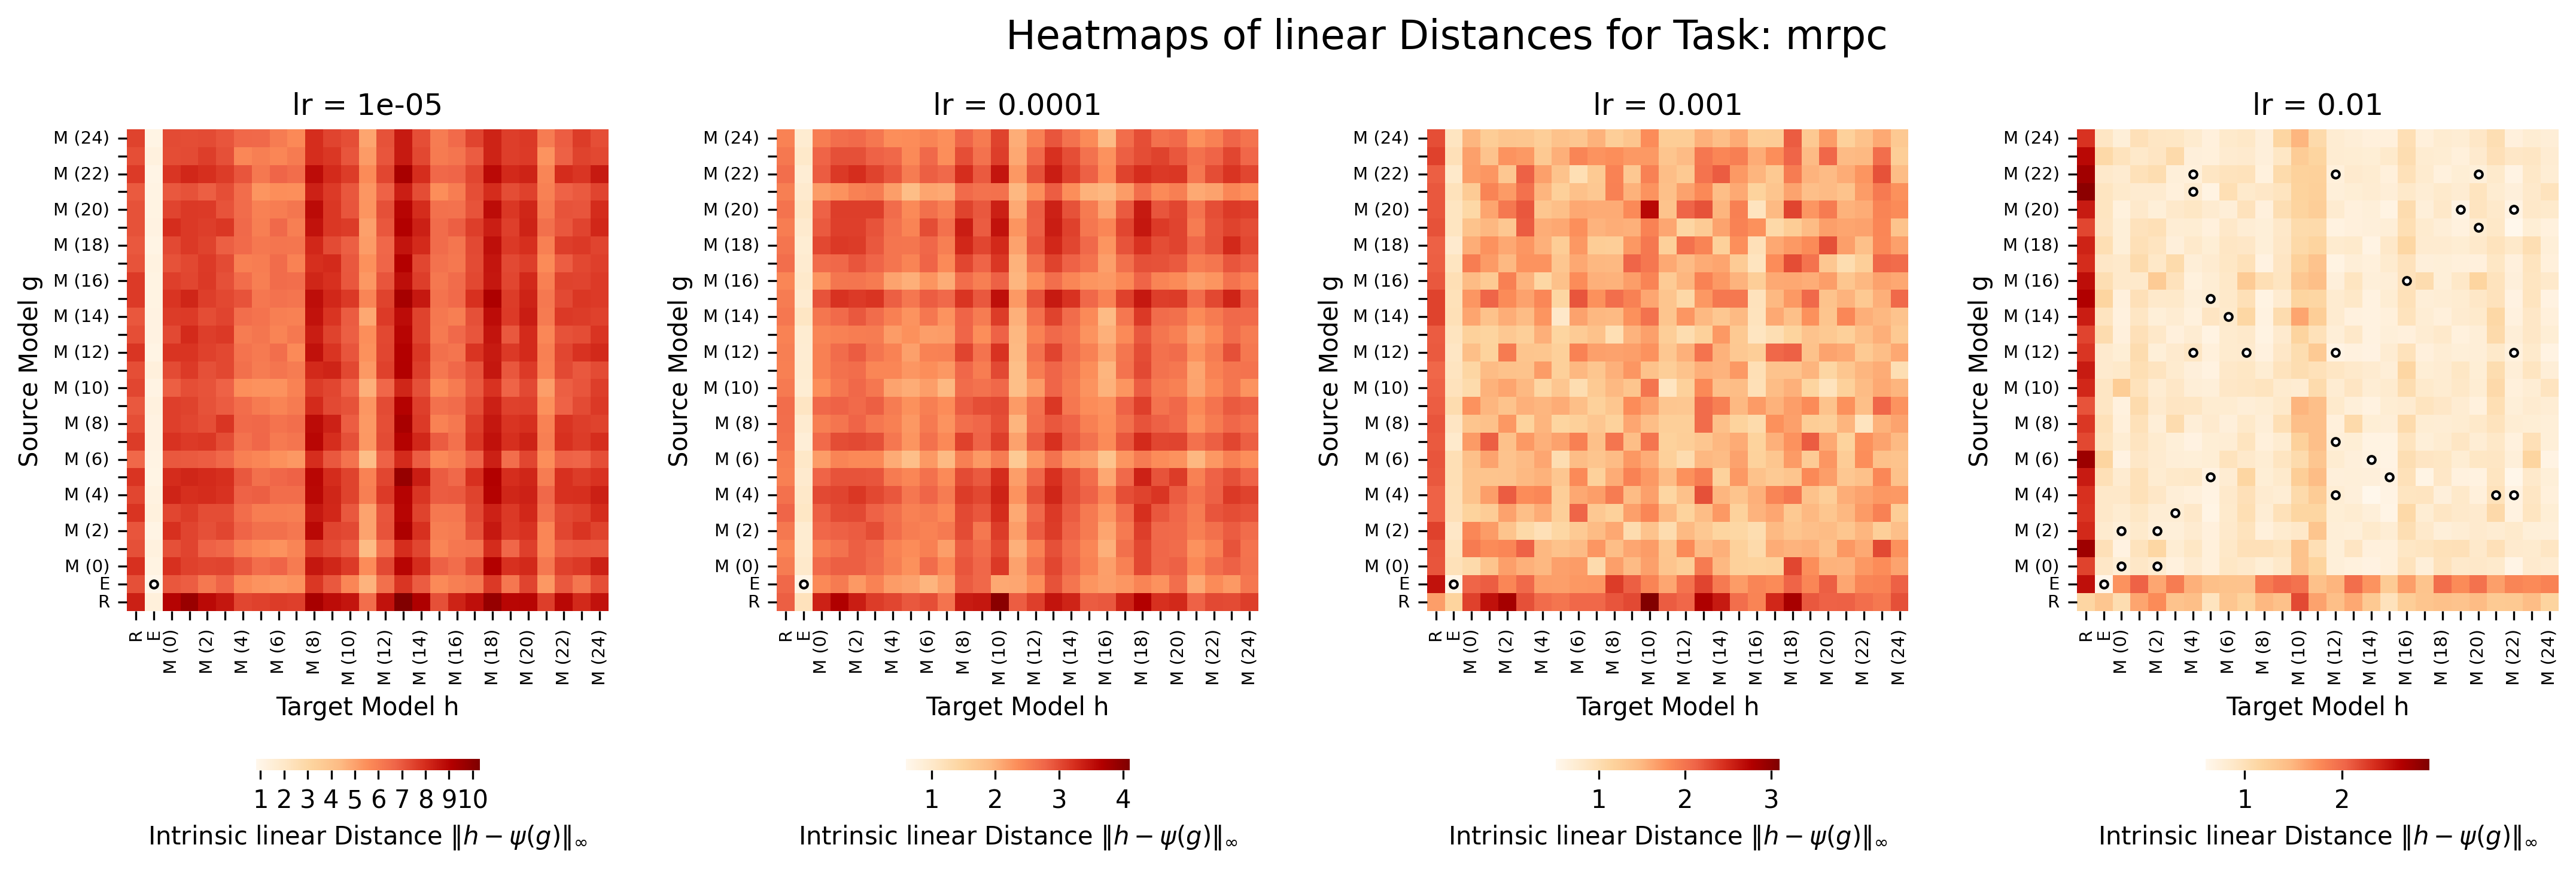
\includegraphics[width=\linewidth]{Abschlussarbeit/Pictures/heatmaps_smaller_circles/Heatmap_linear_distance_all_lrs_mrpc_homotopy.png}
	\caption{Heatmaps of intrinsic distances for affine models on MRPC across learning rates. Pairs with intrinsic distance $<1$ are circled.}
	\label{fig:lin_intrinsic_model}
\end{figure}

\begin{figure}[H]
	\centering
	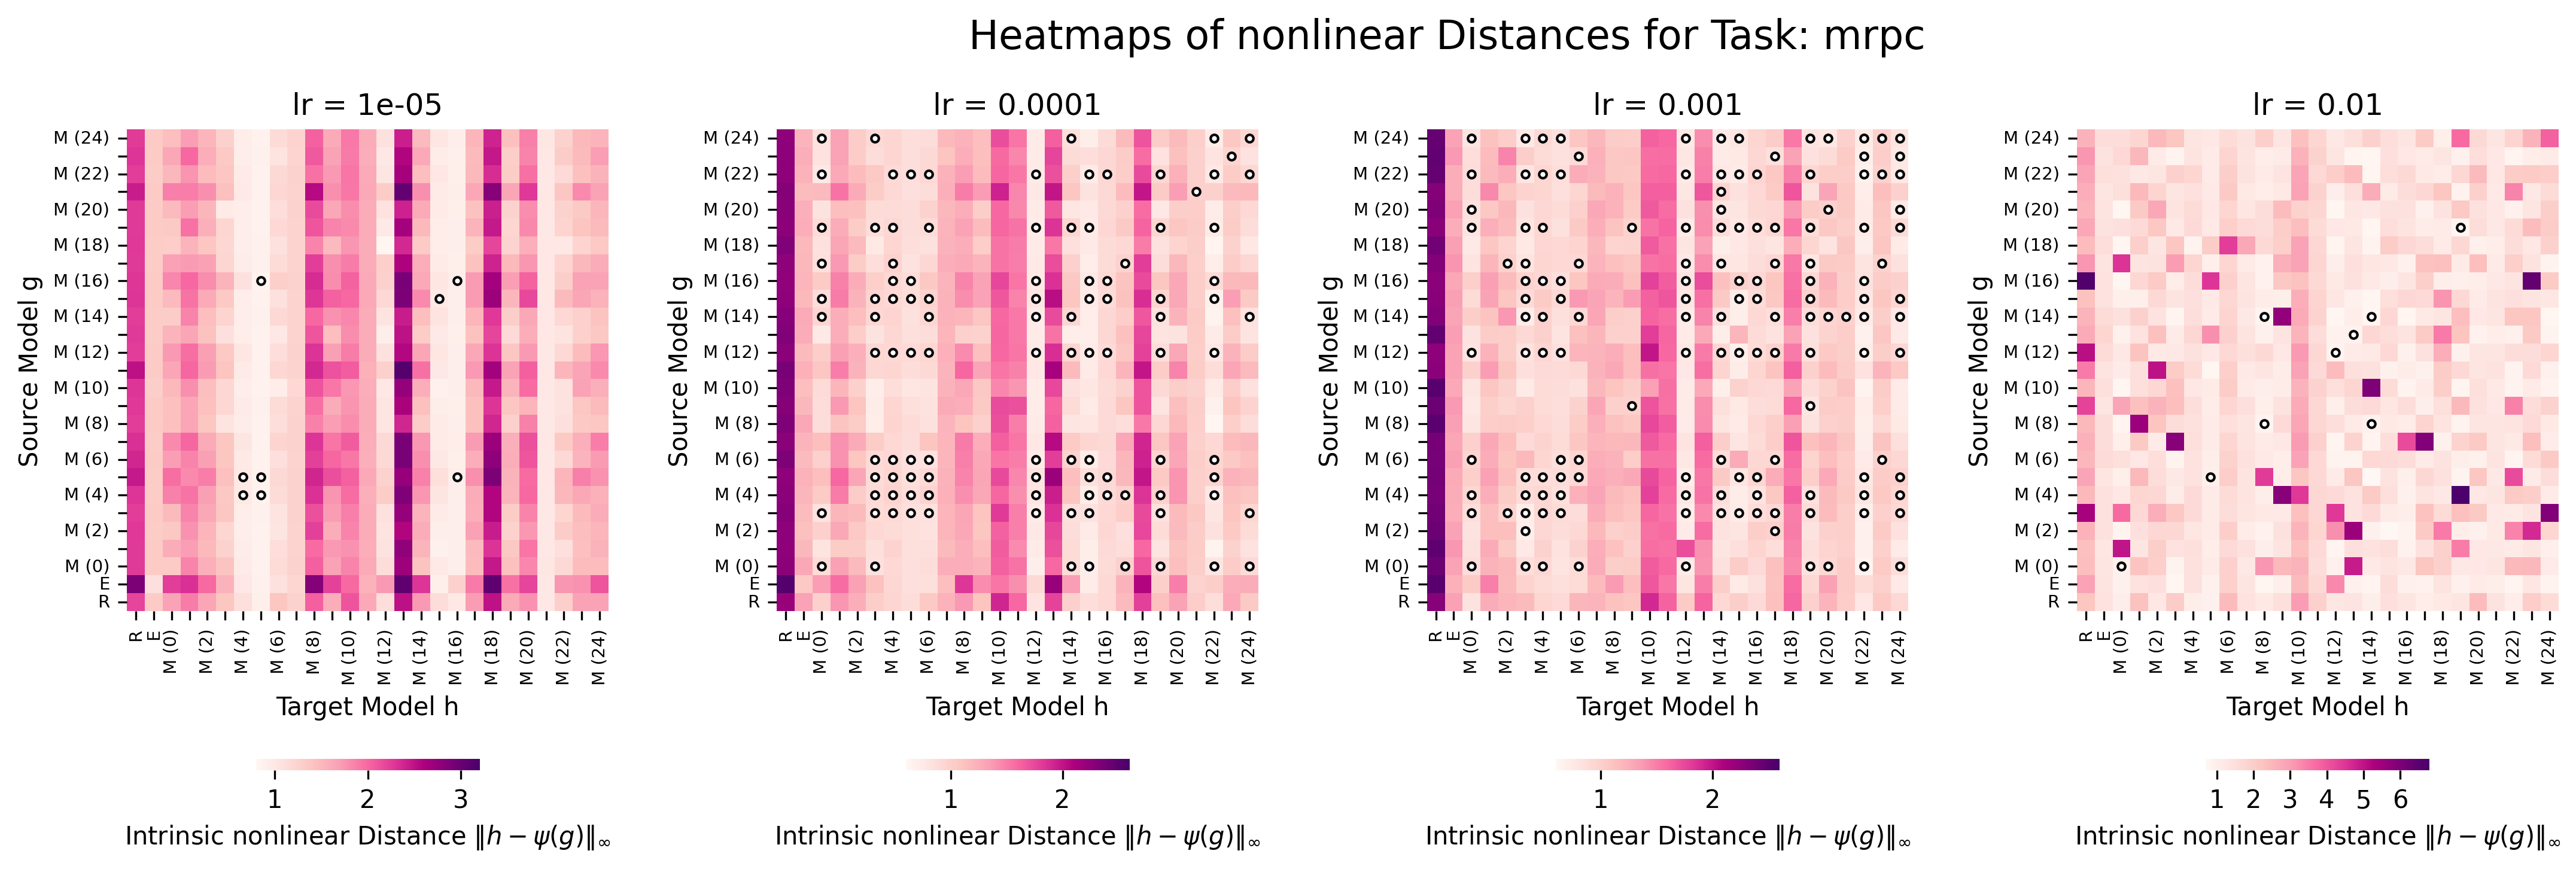
\includegraphics[width=\linewidth]{Abschlussarbeit/Pictures/heatmaps_smaller_circles/Heatmap_nonlinear_distance_all_lrs_mrpc_homotopy.png}
	\caption{Heatmaps of intrinsic distances for non-linear models on MRPC across learning rates. Pairs with intrinsic distance $<1$ are circled.}
	\label{fig:nonlin_intrinsic_model}
\end{figure}

Across all learning rates, we observe that non-linear transformations yield substantially more homotopic model pairs, especially at lower learning rates.  
This supports our previous findings from Figure~\ref{fig:lin_vs_nonlind_dist} and Table~\ref{tab:correlation-transposed}: non-linear models not only achieve smaller average distances but also induce denser and more coherent homotopy structures among encoders.

At higher learning rates, however, both model classes exhibit fewer such pairs, reflecting training instability and diminished approximation quality.  
This reinforces the earlier observation that effective representation alignment critically depends on proper learning rate tuning, particularly for complex transformation classes such as \( \mathcal{F}_{\text{Lip}_1} \).


